\documentclass[english,169,helvet]{ICEbeamerTUMCD}
% options: 169, 1610, 43, mathTUMCD, english, german, ngerman, helvet
% Unknown options are passed to beamer class, e.g., pass t for top alignment of slide content

\newcommand{\PersonTitel}{}
\newcommand{\PersonVorname}{Hedongliang}
\newcommand{\PersonNachname}{Liu}
\newcommand{\PersonStadt}{Munich}
\newcommand{\PersonAdresse}{%
    Theresienstr. 90\\%
    80333~\PersonStadt%
}
\newcommand{\PersonTelefon}{@Telefon@}
\newcommand{\PersonEmail}{@E-Mail@}
\newcommand{\PersonWebseite}{@Web@}
% Fakultät:
\newcommand{\FakultaetName}{Department of Electrical and Computer Engineering}
\newcommand{\LehrstuhlName}{Institute for Communications Engineering}

\hyphenation{} % eigene Silbentrennung
%%%%%%%%%%%%%%%%%%%%%%%%%%%%%%%%%%%%%%%%%%%%%%%%%%%%%%%%%%%%%%%%%%%%%%%%%%%%%%%%


\newcommand{\Datum}{\today}%{July 11, 2019}%


\title{Example presentation}
\author{\PersonVorname{} \PersonNachname{}\inst{1} Another Author\inst{2}}
\institute[]{\inst{1}Technical University of Munich \\ Institute for Communications Engineering
\and \inst{2} Another Institute}
\subject{Thema der Präsentation}


\begin{document}
\setlength{\baselineskip}{\PraesentationAbstandAbsatz}
\setlength{\parskip}{\baselineskip}
% \let\thefootnote\relax\footnote
\PraesentationMasterStandard

\PraesentationTitelseite % Fügt die Startseite eon

\begin{frame}{Overview}
  \tableofcontents[hidesubsections]
\end{frame}
% \section{Structure of a presentation (example)}
% \begin{frame}{Structure of a presentation (example)}
%   \tableofcontents[currentsection, hideothersubsections]
% \end{frame}

\section{Motivation}
\begin{frame}{Motivation}
  \textit{``I will start by giving you a motivation, why ... is interesting in general and why people use it.''}
  \begin{itemize}
  \item Item 1
  \item Item 2
  \item Item 3
  \item ...
  \end{itemize}
  \begin{egbox}{Wonderful Example...}
    This is the example box...
  \end{egbox}
\end{frame}

\begin{frame}{Related Works}
  \textit{``This topic has been studied by...'' / ``Previous results are presented in...''}
  \begin{itemize}
  \item Authors, year\footnote{reference in IEEE style}
  \item Wyner (1974)\footnote{A. Wyner, "Recent results in the Shannon theory," in IEEE Transactions on Information Theory, vol. 20, no. 1, pp. 2-10, January 1974, doi: 10.1109/TIT.1974.1055171.}
  \end{itemize}
\end{frame}
\section{Basics/Prelimenarie}
\begin{frame}{Basics/Prelimenariesw}
  \textit{``The following notations/definitions are needed for ...'' }\\
  This part can contain but not limited to
  \begin{itemize}
  \item Notations
  \item Definitions
  \item Background knowledge
  \item Experimental setups
  \item ... 
  \end{itemize}
\end{frame}

\section{Main contents}
\begin{frame}{Main contents}
  Main contents of a presentation depend on the topic and what you want to convey to the audience. \\The main contents of technical talk could be but not limited to
  \begin{itemize}
  \item a scheme, a method, a construction
  \item a survey, comparisons
  \item experimental results
  \item ...
  \end{itemize}
\end{frame}
\begin{frame}{Illustration with figures}
  \begin{minipage}[t]{0.5\linewidth}
    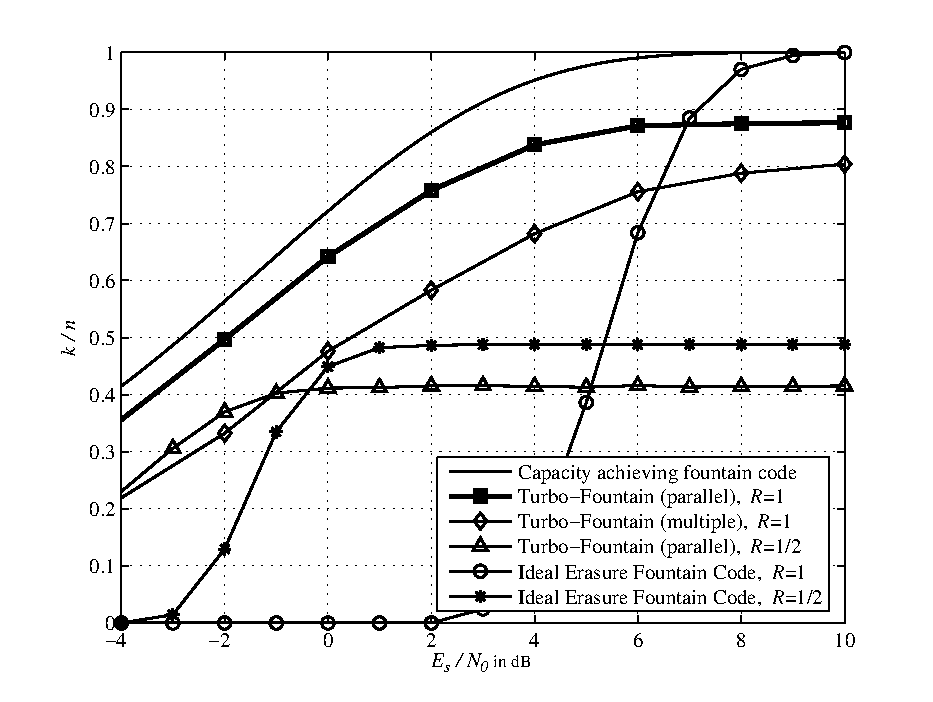
\includegraphics[width=\linewidth]{figs/plot_tf}
  \end{minipage}%
  \begin{minipage}[t]{0.5\linewidth}
    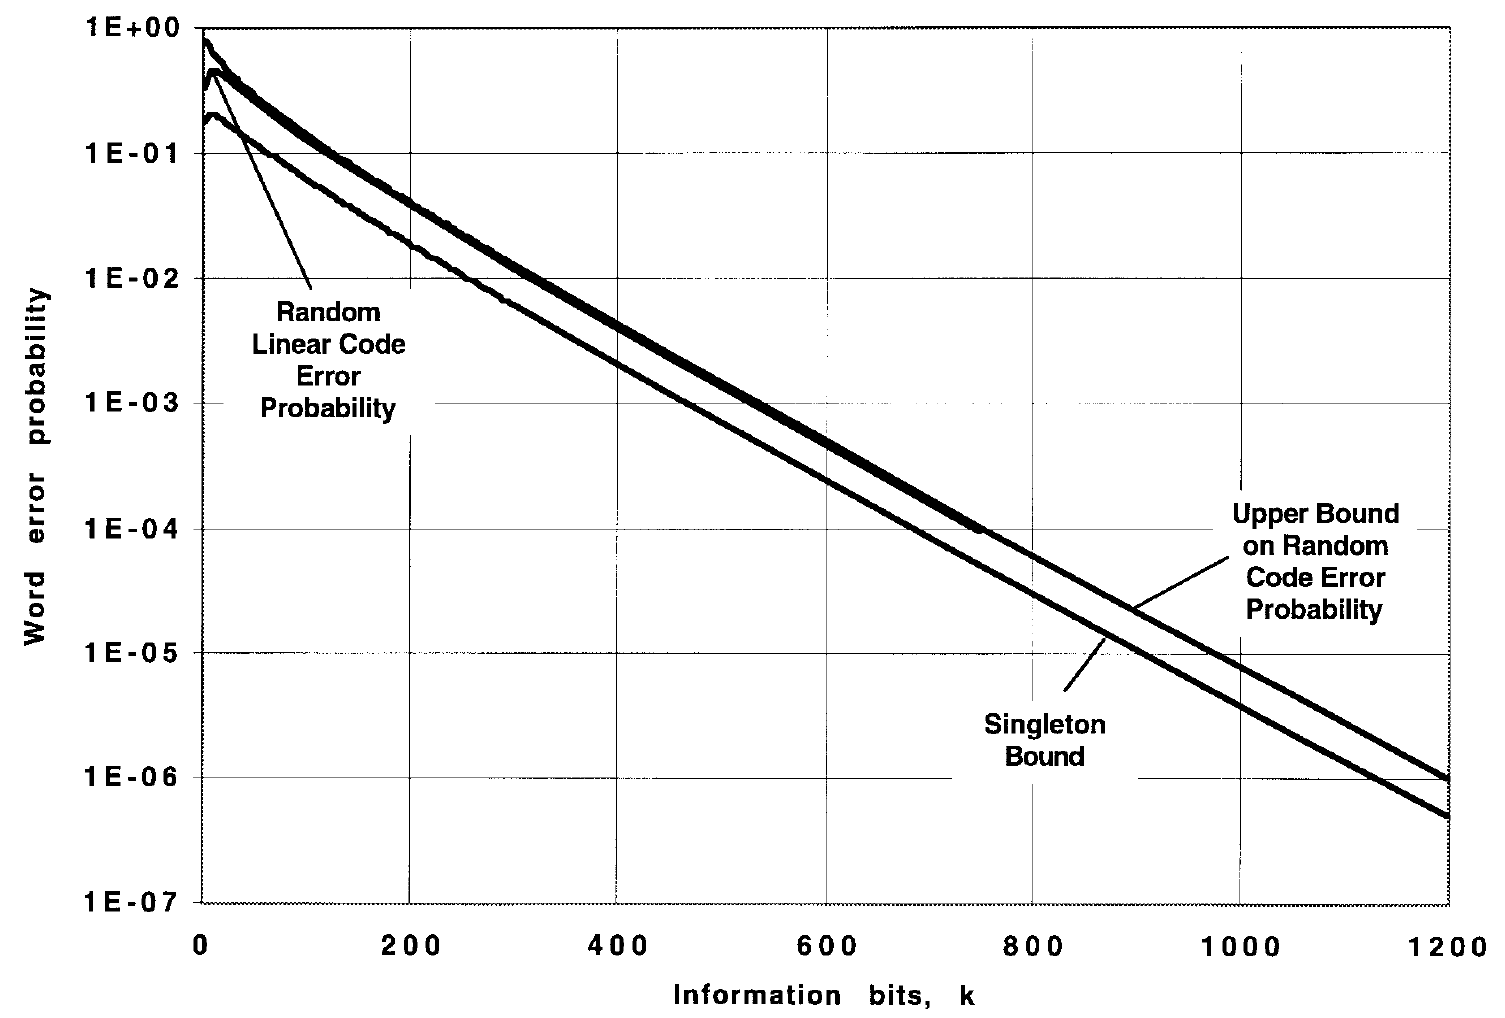
\includegraphics[width=\linewidth]{figs/boundBEC}
  \end{minipage}
  \textit{``From the plots, we can see that...''/ ``The plots show that ...''}
\end{frame}

\section{Conclusion/Summary}
\begin{frame}{Conclusion/Summary}
  \begin{itemize}
  \item \textit{``The conclusion from this work is ...''}
  \item \textit{``The main contributions of this work are ...''}
  \item \textit{``I have talked about ... in this talk.''}
  \end{itemize}
\end{frame}

\appendix
\section{Usage of this template}
\begin{frame}{Appendix: Usage of this template}
  \tableofcontents[currentsection, hideothersubsections]
\end{frame}

\subsection{Basics}
\begin{frame}{Basics}
  \begin{itemize}
  \item This presentation is an adapted version of the TUM corporate design template.
  % \item Instead of many .tex files it is now a self-contained class.
  \item To get it running, you require the file ICEbeamerTUMCD.cls and the folder ``./ressources''
  % \item It's still horrible, but a little less than before.
  \end{itemize}
\end{frame}
\subsection{Useful Environments}
\begin{frame}{Useful environments - Boxes}
    \begin{bluebox}{A blue box}
      Nice to highlight stuff, e.g., theorems, etc.
    \end{bluebox}
    \begin{orangebox}{An orange box}
      Comes in four stylish colors.
    \end{orangebox}
    \begin{greenbox}{A green box}
      Surprisingly, this command gives a green box.
    \end{greenbox}
    \begin{darkbluebox}{Another blue box}
      Slightly darker blue box
    \end{darkbluebox}
\end{frame}

\begin{frame}{Environment Boxes}
    \begin{thmbox}{Important Stuff}
      Same as \emph{bluebox}, but with Theorem in the titlebox.
    \end{thmbox}
    \begin{defbox}{Define Stuff}
      Same as \emph{orangebox}, but with Definition in the titlebox.
    \end{defbox}
    \begin{egbox}{Exemplary Stuff}
      Same as \emph{greenbox}, but with Example in the titlebox.
    \end{egbox}
\end{frame}

\subsection{Page Format}

\begin{frame}{Page Format - Aspect Ratios}
  \begin{itemize}
  \item There are several different aspect ratios to choose from:
    \begin{itemize}
    \item 16:9
    \item 16:10
    \item 4:3
    \end{itemize}
    \item To choose one, pass it as an option to the class (see first line), without the ``:''.
  \end{itemize}
  \begin{minipage}{0.5\linewidth}
    In 16:9 and 16:10 slides are pretty wide.
  \end{minipage}%
  \begin{minipage}{0.5\linewidth}
    So it often makes sense to split them vertically.
  \end{minipage}
\end{frame}

\subsection{Colors \& Fonts}


\begin{frame}{Colors}
  \begin{itemize}
  \item The TUM colors and some additional colors ``similar in style'' are available
    \begin{itemize}
    \item \color{TUMBlau} \emph{TUMBlue / TUMBlau} - Pantone 300
\item \color{TUMBlauDunkel} \emph{TUMBlueDark / TUMBlauDunkel} - Pantone 301
\item \color{TUMBlauHell} \emph{TUMBlueLight / TUMBlauHell} - Pantone 283
\item \color{TUMBlauMittel} \emph{TUMBlueMedium / TUMBlauMittel} - Pantone 542
\item \color{TUMElfenbein} \emph{TUMIvory / TUMElfenbein} - Pantone 7527
\item \color{TUMGruen} \emph{TUMGreen / TUMGruen} - Pantone 383
\item \color{TUMGruenDunkel}\emph{TUMGreenDark / TUMGruenDunkel}
\item \color{TUMOrange}{RGB} \emph{TUMOrange} - Pantone 158
\item \color{TUMGrau} \emph{TUMGrey / TUMGrau} - Grau 60
\item \color{TUMRot} \emph{TUMRed / TUMRot}
    \end{itemize}
  \end{itemize}
\end{frame}

\begin{frame}{Fonts}
  \textbf{Math Font:}\\
  If you really want, use the TUMCD math font (passing mathTUMCD enables the package mathptmx). It doesn't look nice so it's disabled by default.

  Most noticeable with calligraphic letters like $\mathcal{C}$ and $\mathcal{D}$.\\[1em]

  \textbf{Text Font:}\\
  The TUM CD template uses Helvetica, but some might prefer to stick with the \emph{lmodern} font of the LNT templates. If you want to use Helvetica, pass the option \emph{helvet} to the class.\footnote{Also, footnotes leave more space beneath them now.}
  
\end{frame}

%%%%%%%%%%%%%%%%%%%%%%%%%%%%%%%%%%%%%%%%%%%%%%%%%%%%%%%%%%%%%%%%%%%%%%%%%%%%%%%%
\end{document} % !!! NICHT ENTFERNEN !!!
%%%%%%%%%%%%%%%%%%%%%%%%%%%%%%%%%%%%%%%%%%%%%%%%%%%%%%%%%%%%%%%%%%%%%%%%%%%%%%%%
